\documentclass[tikz,border=10pt]{standalone}
\usepackage[utf8]{inputenc}
\usepackage{amsmath, amssymb}
\usetikzlibrary{arrows.meta, positioning, calc, quotes, angles}

\begin{document}

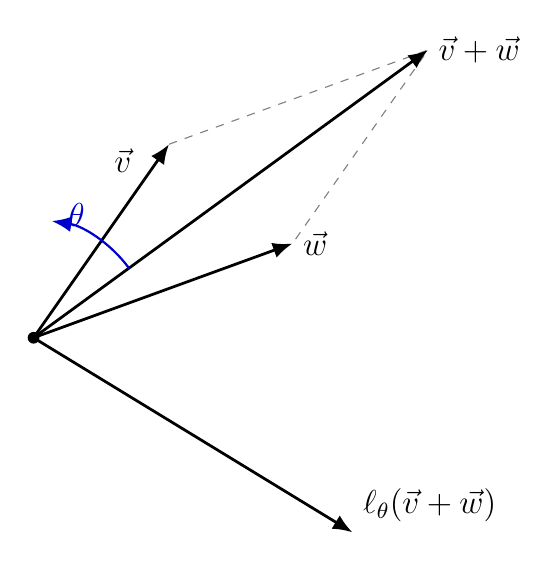
\begin{tikzpicture}[
    thick,
    >={Latex[length=2.5mm, width=2mm]}, % Use your defined arrowheads
    dot/.style={circle, fill=black, inner sep=1.5pt, outer sep=2pt}, % Your dot style
    vector/.style={->, line width=1pt},
    helper/.style={dashed, gray, thin},
    rotation arc/.style={->, blue!80!black, thick}
]

    % === Define Coordinates ===
    \coordinate (O) at (0,0);
    
    % Define vectors v and w (polar coordinates for easier visual control)
    \coordinate (w) at (20:3.5);  % Vector w at 20 degrees, length 3.5
    \coordinate (v) at (55:3.0);  % Vector v at 55 degrees, length 3.0
    
    % Calculate sum v + w
    \coordinate (sum) at ($(v)+(w)$);
    
    % Define rotation angle theta
    \def\thetaAngle{45}
    
    % Calculate the rotated vector l_theta(v+w)
    % Syntax: ($(coordinate)!scale!angle:(origin)$)
    \coordinate (rotated_sum) at ($(sum)!1!\thetaAngle:(O)$);

    % === Draw Parallelogram Construction (Summation) ===
    \draw[helper] (v) -- (sum) -- (w);

    % === Draw Vectors ===
    % Vector w
    \draw[vector] (O) -- (w) node[right, font=\large] {$\vec{w}$};
    
    % Vector v
    \draw[vector] (O) -- (v) node[above left, pos=0.8, font=\large] {$\vec{v}$};
    
    % Vector Sum
    \draw[vector] (O) -- (sum) node[right, font=\large] {$\vec{v} + \vec{w}$};

    % === Draw Rotated Vector ===
    \draw[vector] (O) -- (rotated_sum) node[above right, font=\large] {$\ell_\theta(\vec{v} + \vec{w})$};

    % === Draw Rotation Angle theta ===
    % We use the 'angles' library logic manually or via arc for precise control
    % Calculate the angle of the sum vector relative to x-axis
    \pgfmathanglebetweenpoints{\pgfpointanchor{O}{center}}{\pgfpointanchor{sum}{center}}
    \let\startAng\pgfmathresult
    
    % Draw the arc from sum to rotated sum
    \draw[rotation arc] ($(O) + (\startAng:1.5)$) 
        arc [start angle=\startAng, end angle=\startAng+\thetaAngle, radius=1.5]
        node[midway, above left, font=\large] {$\theta$};

    % === Draw Origin Dot ===
    \node[dot] at (O) {};

\end{tikzpicture}
\end{document}
